\chapter{Research method}

\section{Scenarios}


To conduct this research we have created some fictitious scenarios that we can run against a custom made domain reasoner or an existing domain reasoner.
The first scenario represent some exercises executed bij a fast student. 
This is the happy flow where everything goes well.
The second scenario is a normal student, who also attempt some exercises that fail.
The third scenario is a slow student. 
He has some learning problem. 
The \gls{its} must diagnose this and offer support. 


A scenarios is a serie request/response cycles, that simulate a student dialogue.
These messages are written in a student log, which is the basis to experiment with reasoning about student progress and knowledge.

From these traces we derive an educational model as a first step and a student knowledge model as a second step.
The educational meta-model describes the \gls{its} in terms of available exercises and task classes.
The educational student model describes the the progress of the student in the curriculum in terms of exercises and task classes completed successfully.
As a second step we reason about student knowledge and skills.
We use an ontology model and a rule system to do most of the reasoning.


\section{Educational Model}

The educational model describes the curriculum, in terms of task classes,  learning tasks available and their definitions.
The model also describes the history of the learners actions in terms of learning tasks executed and the individual steps in each task.

This model captures the logging of the student learning actions, in as much detail as possible.
The purpose is just to create a recording of the student actions, from which we can derive the student model.

A relational database would be an obvious choice for a production ready \gls{its}.
However we want to experiment with the reasoning and inferencing of the student model and interventions.
For this purpose we use an ontology model to store the student log.
The ontology model is loaded with the student data as presented below.
And as an optimisation some trivial derived facts are added.
For example object properties (binary relationships) from key relationships, and some counters.




\subsection{The student log model}
\begin{table}[H]
\begin{tabular}{| l | l | r |}
\hline
Field & Description\\
\hline
tcdKey & primary key\\
tcdName & Task class name\\
\hline
\end{tabular}
\caption{Taskclass definition (tcd)}
\label{Taskclass}
\end{table}


\begin{table}[H]
\begin{tabular}{| l | l | r |}
\hline
Field & Description\\
\hline
ltdKey & Primary key\\
tcdRef & Reference to which task class the task belongs.\\
ltdName & Name for the learning task\\
ltdDescription & Description of the exercise\\
ltdExerciseId & Name of the exercise in the domain reasoner\\
ltdDifficullty & Level of difficulty: VeryEasy Easy Medium Difficult, VeryDifficult \\
ltdStartExpression & The start expression of the exercise\\
\hline
\end{tabular}
\caption{Learning task definition (ltd)}
\label{Learning task definition}
\end{table}

 
\begin{table}[H]
\begin{tabular}{| l | l | r |}
\hline
Field & Description\\
\hline
lteKey & Primary key \\
ltdRef & Reference to learning task definition\\
completed & The task was successfully completed\\
givenUp & The student started another exercise without finishing this one.\\
steps & The number of learning steps executed\\
counters & A list of counters on number of errors and rule executions\\
\hline
\end{tabular}
\caption{Learning task execution (lte)}
\label{Learning task execution}
\end{table}
 
\begin{table}[H]
\begin{tabular}{| l | l | r |}
\hline
Field & Description\\
\hline
tseKey & Primary key \\
lteRef & Reference to learning task definition\\
tseAction & The (inter)action with the domain reasoner, a request/response cycle.\\
\hline
\end{tabular}
\caption{Task step execution (tse)}
\label{Task step execution}
\end{table}

The tseKey is the sequence number of the task steps. 
Task steps are numbered sequentially. e.g tse 1-15 belong to lte 1;  tse 16-21 to lte 2 etc.
 The most important actions are a create and a diagnose action.

A create action specifies and exerciseId recognised by the domain reasoner and a start expression.
Domain reasoners often contain already a list of such exercises including their difficulty.
This can be used to load the model with an initial set of learning task definitions.

A diagnose action contains an expression submitted by the student.
The system responds a diagnostic result, including which rule was applied and a finished indicator.



\begin{table}[H]
\begin{tabular}{| l | l | l |}
\hline
Action & Input & result\\
\hline
Create & exerciseId, start expression & \\
Diagnose & expression & Syntax\\
Diagnose & expression & Buggy\\
Diagnose & expression & NotEquivalent\\
Diagnose & expression & Similar, finished\\
Diagnose & expression & WrongRule, finished\\
Diagnose & expression & Expected, finished, stepRule\\
Diagnose & expression & Detour, finished\\
Diagnose & expression & Correct, finished\\
\hline
\end{tabular}
\caption{Task step actions and results}
\label{Task step actions}
\end{table}

\section{Scenario: the fast student}

To demonstrate the working of the student model  we work with fictive cases of student logs.
The logs have been produced by running a series of requests through a domain reasoner, the results transformed into the model and an ontology model.
The first task class is modeled after chapter 1 of the textbook \citep{hutton_2016}.
This chapter presents a casus of a very simple function:
\vspace{10pt}

$double  \hspace{5 pt} x = x + x$
\vspace{10pt}

To get more variation we added a maximum function including ''if'' and ''greater then''.

\begin{figure}
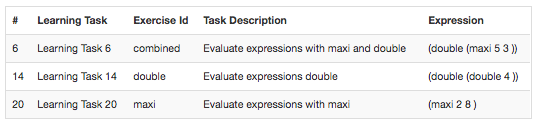
\includegraphics[scale=0.85]{pictures/screen01.png}
\caption{Part of task class}
\label{fig:screen01}
\end{figure}

Figure \ref{fig:screen01} show the subset of this task class used in our first scenario a fast student.
This scenario is a the simplest as it is in fact a happy flow, without need for interventions.

\begin{figure}
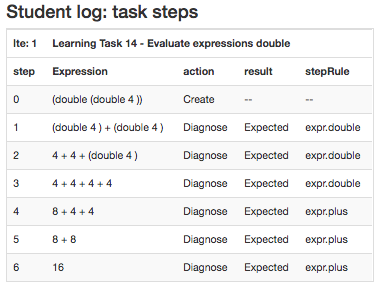
\includegraphics[scale=1.0]{pictures/screen02.png}
\caption{Trace}
\label{fig:trace01}
\end{figure}
In figure \ref{fig:trace01} we see the trace of the first exercise.
In step 0 a create message was send to the domain reasoner to just start the exercise.
In step 1 the student took as a first step to substitute the outer ''double''.
In the next steps the other doubles are substituted and step by step the numbers added.

In each step we executed a diagnose action that in this happy flow gave a result ''expected''. 
For each step the steprule was returned.
For this exercise there are only two rules relevant: ''expr.double'' and ''expr.plus''.
The names of the rules are determined in the code of the domain reasoner.
The reasoner recognises which rule was applied.

The last step returned also a field ''finished'' with value true, the other steps false.
This is not shown in the trace.
In each transmission we also send and receive some additional data that represents where we are in the exercise.
Since the domain reasoner is stateless, the client has to keep track of this state.
This data is not used in the student model, and not shown.

\begin{figure}
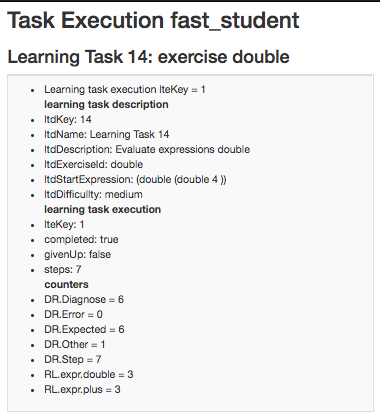
\includegraphics[scale=1.0]{pictures/screen03.png}
\caption{Results of the first task execution}
\label{fig:lte01}
\end{figure}

In figure \ref{fig:lte01} we see some of the data mentioned in the model description.
The name and number of the exercise, start expression are part of the learning task definition.

The picture show the data from the exercise that we executed.
The first fields describe the learning task definition.
The next part show the learning task execution.
The lteKey is assigned in sequential ordering, so this is number one.
The exercise was completed, inferred from the last task step that had flag finished on true.
There were seven steps executed including the create.

The counters are divided in generic domain reasoner counters (DR) and rule executions (RL).
The number of errors is the sum of the Syntax, Buggy, NotEquivalent, and WrongRule diagnose results.
The model can off coarse be refined to include the individual counters.
We pre-calculate some facts, to simplify the ontology. 

\section{Inferencing in the ontology}
\label{section:infont}
In this first scenario we show how we can define whether an exercise is completed successfully.
This must then be formalised in rules.
We formulate the following criteria for successful completion of individual exercises:
\begin{itemize}
\item An exercise must be completed without errors. 
\item The student must have applied a certain number of rules, in the previous case ''expr.double'' and ''expr.plus'' must be executed at least once.
\item The student must have completed the exercise, as indicated by the domain reasoner. 
\end{itemize}



\begin{figure}
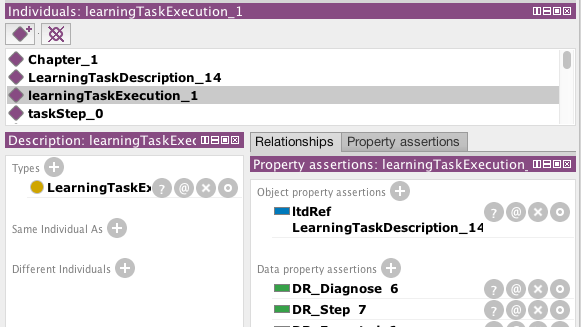
\includegraphics[scale=0.7]{pictures/screen07.png}
\caption{Some individuals in the ontology}
\label{fig:onto04}
\end{figure}

Figure \ref{fig:onto04} show a screenshot of Prot\'eg\'e, a tool to edit an ontology model.
An ontology model contains individuals about which facts can be asserted or inferred.
Figure \ref{fig:onto04} shows some of the individuals that we have seen before.
The individual identified as  ''learningTaskExecution\_1'' represents the learning task execution shown before.
The properties show in figure \ref{fig:lte01} are data properties.
The relationships between individuals defined with keys now become object properties.
The relationship ltdRef connects ''learningTaskExecution\_1'' to '' LearningTaskDescription\_14''.
This ltdRef and other relations are subrelations of partOf, a transitive relation.
The reasoner can then infer everything that is ''partOf'' the task class, including the steps.
A relation ''hasPart'' is defined as the inverse of ''partOf''.



\begin{figure}
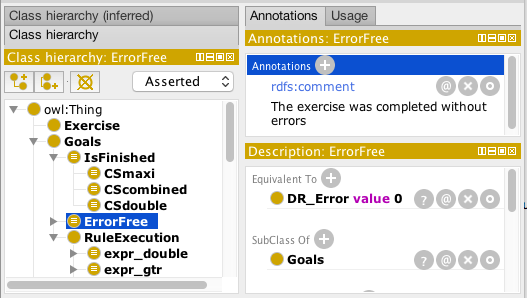
\includegraphics[scale=0.7]{pictures/screen04.png}
\caption{Ontology definition for ErrorFree}
\label{fig:onto01}
\end{figure}

Classes and subclasses are an important concept in reasoning. 
A class plays the role of an unary predicate. We like our learning task execution to be member of ErrorFree, which is equivalent to having zero errors.


\begin{figure}
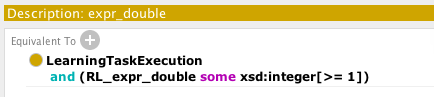
\includegraphics[scale=0.7]{pictures/screen05.png}
\caption{Ontology definition for rule expr.double}
\label{fig:onto02}
\end{figure}

Screenshot \ref{fig:onto02} shows a similar definition of the class expr\_double equivalent to rule ''expr.double'' must be executed at least once.
Similar defnitions can be made for the other conditions. 
When a reasoner is run, it will infer class membership from the data properties show before.



\begin{figure}
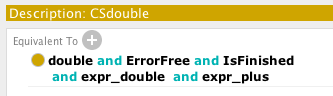
\includegraphics[scale=0.7]{pictures/screen06.png}
\caption{Ontology definition for class CSDouble}
\label{fig:onto03}
\end{figure}
To determine if the exercise double was completed successful a class CSdouble is defined as shown in figure \ref{fig:onto03}.
The criteria are that the it must have an exerciseId ''double'', error free, finished, and the rules ''expr.double'' and ''expr.plus'' must have been applied at least once. This is the formal definition of the criteria we formulated in the beginning of this section.

\begin{figure}
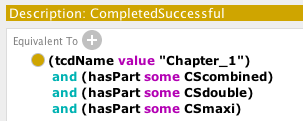
\includegraphics[scale=0.7]{pictures/screen08.png}
\caption{Completed Succesfull criteria for Chapter 1}
\label{fig:onto05}
\end{figure}

We have seen in subsection \ref{procsupport} that the learner may proceed to the next task class when no more support is needed.
As criterium for successful task class completion of task class 1 we specify one successful completion of each exercise double, maxi and  combined.
In figure \ref{fig:onto05} the formal definition of this definition is shown. 

The exercise combined uses the same ruleset as double and maxi together. 
So a lighter criterium could be that either combined must be executed or else both maxi and double.
It is up to the \gls{its} designer to formulate criteria for success or failure.
Here we show how such criteria can be translated in formal business rules of the student model.
It must be anticipated that rules like this get more and more refined as more experience is gained with the \gls{its} in practice.
A business rule engine offers a flexible way to adapt these rules, which is important for the evolution of the \gls{its}.


\begin{figure}
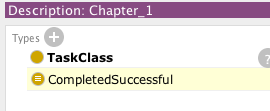
\includegraphics[scale=0.7]{pictures/screen09.png}
\caption{Chapter 1 inferred as completed successful}
\label{fig:onto06}
\end{figure}

Figure \ref{fig:onto06} shows that the reasoner inferred that the individual Chapter 1 is member of the class CompletedSuccessful.
An inferred fact is shown with a yellow background in Prot\'eg\'e.
Thus, the fast student successfully completed the exercises and the task class.
If the reasoner runs one step earlier, then the last exercises did not get finished and it is not CompletedSuccessful.

\section{A normal student.}
In the scenario of the fast student we showed that we used counters to calculate student progress.
In this scenario we use the same approach, but normally a student will make some errors.
In fact this is the core business of the \gls{its} as this student probably learns more from his errors.
Let us see what happens when some errors are made.

\begin{figure}
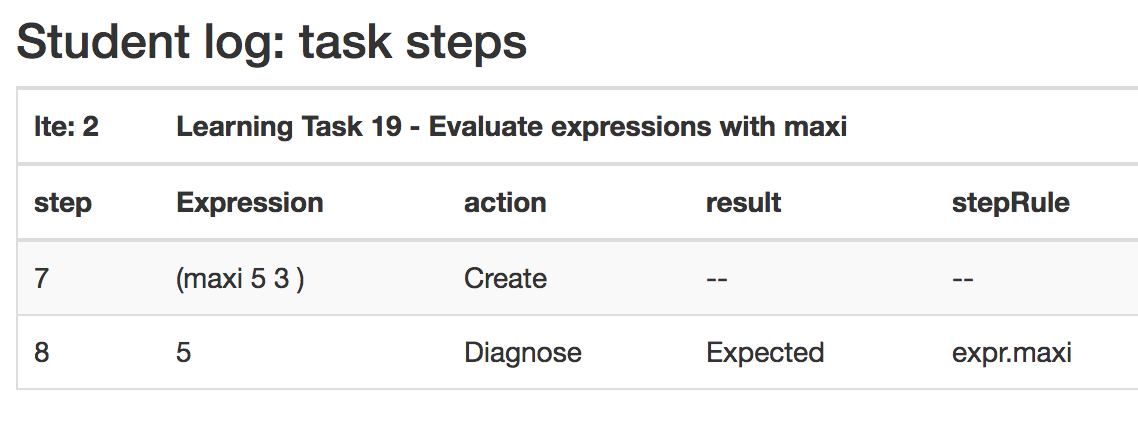
\includegraphics[scale=0.7]{pictures/screen10.png}
\caption{Incomplete exercise}
\label{fig:onto07}
\end{figure}

In figure \ref{fig:onto07} we see a part of the studentlog where the student looked at the expression and just gave the correct answer five.
The idea of the exercise was to practice step by step equational reasoning.
This is not the idea of this exercise. 

\begin{figure}
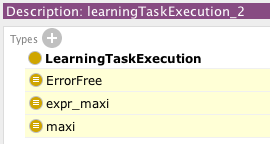
\includegraphics[scale=0.7]{pictures/screen11.png}\\
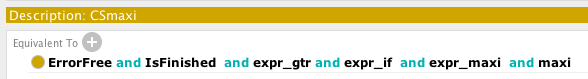
\includegraphics[scale=0.7]{pictures/screen12.png}
\caption{Incomplete exercise}
\label{fig:onto08}
\end{figure}

The definition of CSmaxi includes classes expr\_gtr and expr\_if, but these rules were not executed.
The reasoner has therefore not inferred this exercise as successful (CSmaxi)  \ref{fig:onto08}.


\begin{figure}
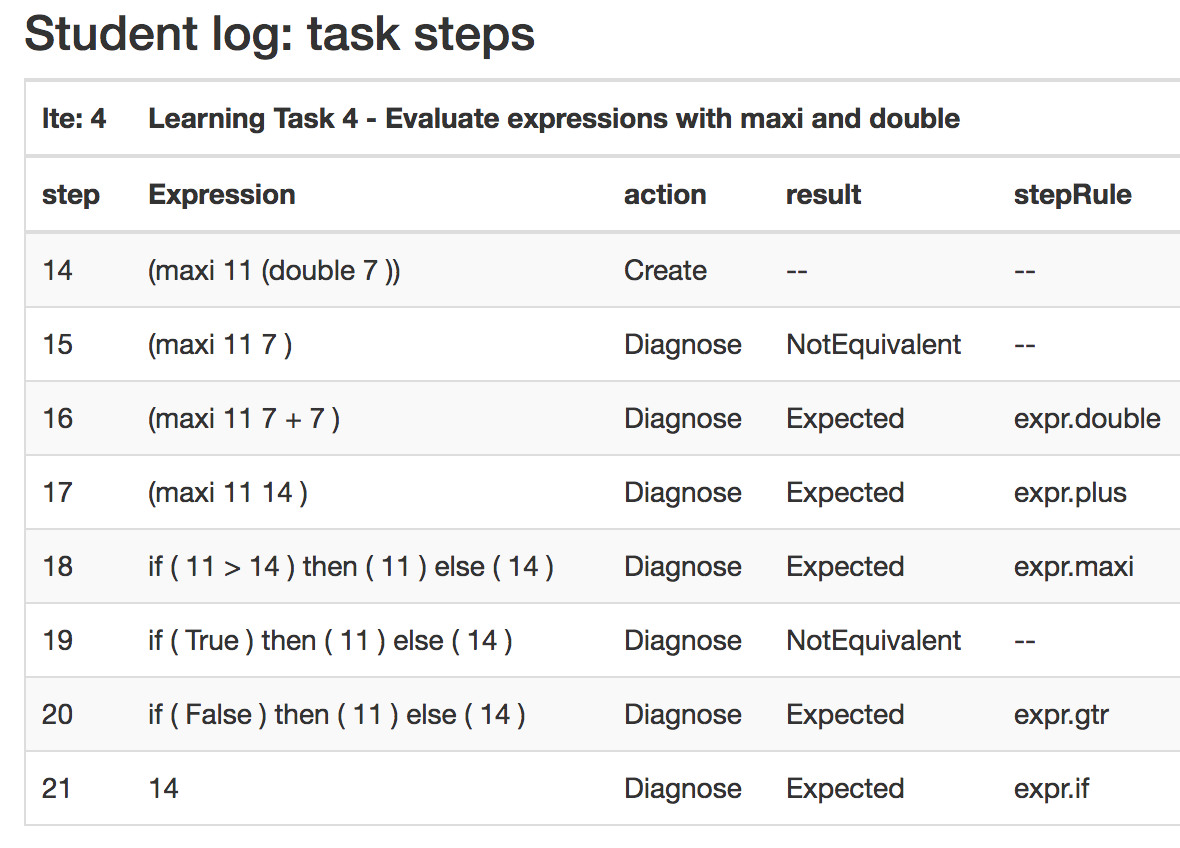
\includegraphics[scale=0.7]{pictures/screen13.png}\\
\caption{Incomplete exercise}
\label{fig:onto09}
\end{figure}

In another exercise the student made a mistake in step 15, he lost the double which should have expanded to ''$7 + 7$''.
The rest of the exercise was completed successful as it is not member of class ErrorFree.
This exercise did not complete successful, as the \gls{its} had to give procedural support.
He has to complete another errorFree exercise to complete the task class.

At such a point there are possibilities to infer an intervention. 
The system might query the domain reasoner to get a list of possible next steps, and find that he missed the rule ''expr.double''.
If the student started with the more complex exercise ''combined'' we could suggest to first complete an exercise double.
In this case we could advice to first execute the exercise double.

Following the TenSteps we could offer part task practices for example with evaluation of comparison operators.
Off course this is a contrived example, but in a programming exercise we could offer small practice tasks on prelude functions.

\section{Reasoning about the domain model}
In the previous sections the reasoning about exercise executions was based on sets of counters for rule executions.
In domain models the term bandwidth is used to denote how much information on the students activity is available \citep{studentModelling}.
In a realistic situation we could also use response times, facial expression, or eye movement taken with the webcam.
We will not go that far, but we can extract more information from a domain reasoner log by analysing the expression that are exchanged.
In ref{c02:mental} we saw some domain concepts in mental models.

By analysing the expressions we can analyse which domain concepts the student encountered in the exercise.
In Ask-Elle and the Haskell Expression evaluator the expressions are parsed into a parse tree.
From the parse tree we can derive what domain concepts play a role, for example recursion.
The student model we use is an overlay model that overlays the domain concept. 
In our case we worked with counters, so we could expand the model with counters for domain concepts such as recursion or high order functions.
In our previous example this would more or less duplicate the findings of rule executions.

It is a design choice which domain aspects are counted this way.
The Haskell expression evaluator has rules name like ''eval.repeat'', ''eval.takewhile'' named after each prelude function.
In that case parsing and counting prelude function occurrences would be redundant with rule execution counts.
Similar in our case the fact that the expression contains a ''+''-sign would duplicate counting the rule ''expr.plus''.

On the other hand must we realise that these counters represent different learning dimensions.
Rule executions are a measure of the student learning rules an building up skills and experience.
Domain concepts relate to schema build-up from materials found in supportive materials.























